\documentclass[a4paper,portrait,columns=3,5pt]{cheatsheet}
\title{Formulario Analisi 2}
%\author{Elena Acinapura, Giacomo Fabris}
\author{}
\date{\today}

\usepackage{commath}
\usepackage{graphicx}
\usepackage{mathtools}
\usepackage{commath}
\usepackage{amssymb}
\usepackage{amsmath}
\usepackage[utf8]{inputenc}

\begin{document}
%\maketitle

\section{Formule trigonometriche}
\subsection{Addizione e sottrazione}
$$\sin (\alpha + \beta) = \sin(\alpha) \cos(\beta) + \cos(\alpha)\sin(\beta)$$
$$\sin(\alpha - \beta) = \sin(\alpha) \cos(\beta) - \cos(\alpha)\sin(\beta)$$
$$\cos(\alpha + \beta) = \cos(\alpha) \cos(\beta) - \sin(\alpha) \sin(\beta)$$
$$\cos(\alpha - \beta) = \cos(\alpha) \cos(\beta) + \sin(\alpha) \sin(\beta)$$
$$\tan(\alpha + \beta) = \frac{\tan(\alpha) + \tan(\beta)}{1 - \tan(\alpha)\tan(\beta)}$$
$$\tan(\alpha - \beta) = \frac{\tan(\alpha) - \tan(\beta)}{1 + \tan(\alpha)\tan(\beta)}$$
\subsection{Duplicazione}
$$\sin(2\alpha) = 2\sin(\alpha)\cos(\alpha)$$
$$\cos(2\alpha) = \cos^2 (\alpha) - \sin^2 (\alpha)$$
$$\tan(2\alpha) = \frac{\tan(\alpha)}{1 - \tan^2(\alpha)}$$
$$\cot(2\alpha) = \frac{\cot^2(\alpha) - 1}{2\cot(\alpha)}$$
\subsection{Bisezione}
$$\sin\left(\frac{\alpha}{2}\right) = \pm \sqrt{\frac{1 - \cos(\alpha)}{2}}$$
$$\cos\left(\frac{\alpha}{2}\right) = \pm \sqrt{\frac{1 + \cos(\alpha)}{2}}$$
$$\tan\left(\frac{\alpha}{2}\right) = {\frac{1 - \cos(\alpha)}{\sin(\alpha)}}$$
$$\cot\left(\frac{\alpha}{2}\right) = {\frac{1 + \cos(\alpha)}{\sin(\alpha)}}$$
\subsection{Werner}
$$\sin(\alpha)\sin(\beta) = \frac{1}{2} \left[\cos(\alpha - \beta) - \cos(\alpha + \beta)\right]$$
$$\cos(\alpha)\cos(\beta) = \frac{1}{2} \left[\cos(\alpha - \beta) + \cos(\alpha + \beta)\right]$$
$$\sin(\alpha)\cos(\beta) = \frac{1}{2} \left[\sin(\alpha - \beta) + \sin(\alpha + \beta)\right]$$

\section{Derivate fondamentali}
$$ (\tan(x))' = 1 + \tan^2(x) = \sec^2(x)$$
$$ (\arcsin(x))' = \frac{1}{\sqrt{1 - x^2}}$$
$$ (\arccos(x))' = - \frac{1}{\sqrt{1 - x^2}}$$
$$ (\arctan(x))' = \frac{1}{1 + x^2}$$
$$ (\sec(x))' = \tan(x)\sec(x)$$
$$ (\csc(x))' = -\cot(x)\csc(x)$$
$$ (\cot^n(x))' = - n \cdot \csc(x) \cdot \sec(x) \cdot \cot^n (x)$$
$$ (a^x)' = a^x \ln(a)$$
$$ (\log_a~x )' = \frac{1}{x\ln(a)}$$

\section{Roba iperbolica}
$$ \sinh(x) = \frac{e^x - e^{-x}}{2} $$
$$\cosh(x) = \frac{e^x + e^{-x}}{2}$$
$$ \cosh^2(x) - \sinh^2(x) = 1 $$
$$ (\cosh(x))' = \sinh(x)$$
$$ \quad (\sinh(x))' = \cosh(x) $$
\section{Sostituzioni notevoli}
\textit{Per funzioni razionali in seno e coseno:} 
$$t \coloneqq tan(\frac{x}{2})\quad \dif x = \frac{2}{1 + t^2} \dif t$$
$$ \sin(x) = \frac{2t}{1+t^2} \quad \cos(x) = \frac{\-t^2}{1+t^2}$$

\textit{Per radici del tipo $\sqrt{a - x^2}$:}
$$ x = \sqrt{a} \sin(t) $$
\section{Disuguaglianze utili}
$$ \abs{xy} \leq \frac{1}{2}\left(x^2 + y^2\right) $$
$$ \abs{\sin(xy)} \leq \abs{xy}\quad \text{per xy$\rightarrow$ 0}$$
\section{Sviluppi in serie}
$$ e^x = 1 + x + \frac{x^2}{2!} + \frac{x^3}{3!} + o(x^3)$$
$$ \ln(1 + x) = x - \frac{x^2}{2} + \frac{x^3}{3} + o(x^3)$$
$$ \sin(x) = x - \frac{x^3}{3!} + \frac{x^5}{5!} + o(x^6)$$
$$ \cos(x) = 1 - \frac{x^2}{2!} + \frac{x^4}{4!} + o(x^5)$$
$$ \tan(x) = x + \frac{x^3}{3} + \frac{2x^5}{15} + o(x^6)$$
$$ \arctan(x) = x - \frac{x^3}{3} + \frac{x^5}{5} + o(x^6)$$
$$ \frac{1}{1-x} = 1 + x + x^2 + x^3 + o(x^3)$$
$$(1 + x) ^ \alpha = 1 + \alpha x + \frac{\alpha (\alpha - 1)x^2}{2!} + \dots $$
$$ + \frac{\alpha(\alpha - 1)\dots (\alpha - n - 1) x^n}{n!} + o(x^n) $$

\section{Integrali utili}
$$ \int \sin^2(x) \dif x = \frac{1}{2} (x - \sin(x) \cos(x)) $$
$$ \int \sin^3(x) \dif x = \frac{1}{12} (\cos(3x)-9\cos(x)) $$
$$ \int \sin^4(x) \dif x = \frac{1}{32} (12x - 8\sin(2x)+\sin(4x)) $$
$$ \int \sin^n(x) \dif x = -\frac{1}{n} \cos(x) \sin^{n-1}(x) + $$ 
$$ + \frac{n-1}{n} \int \sin^{n-2}(x) \dif x $$
$$ \int \cos^2(x) \dif x = \frac{1}{2} (x + \sin(x)\cos(x)) $$
$$ \int \cos^3(x) \dif x = \frac{1}{12} (\sin(3x) + 9\sin(x))$$
$$ \int \cos^4(x) \dif x = \frac{1}{32} (12 x + 8\sin(2x)+\sin(4x))$$
$$ \int \cos^n(x) \dif x = \frac{1}{n} \sin(x) \cos^{n-1}(x) + $$
$$ + \frac{n-1}{n} \int \cos^{n-2}(x) \dif x $$
$$ \int \sin(x) ~ \cos(x) \dif x = -\frac{1}{2} \cos^2(x) $$ 
$$ \int \sec(x) \dif x = \ln (\tan(x) + \sec(x)) $$
$$ \int \sec^2(x) \dif x = \tan(x) $$
$$ \int \csc (x) \dif x = \ln \left( \tan\left(\frac{x}{2}\right)\right)$$
$$ \int \csc^2(x) \dif x = \cot(x) $$
$$ \int \log(f(x)) \dif x = x \log (f(x)) - \int \frac{x}{f(x)} \dif x $$
$$ \int \sqrt{a - x^2} \dif x = \frac{x}{2} \sqrt{a - x^2} + \frac{a}{2} \arcsin \left(\frac {x}{a}\right) = $$
$$ =  \frac{x}{2} \sqrt{a - x^2} + \frac{a}{2} \arctan \left(\frac{x}{\sqrt{a-x^2}}\right) $$
$$ \int \sqrt{a + x^2} \dif x =  \frac{x}{2} \sqrt{a + x^2} + $$ 
$$ + \frac{a}{2} \ln \abs{\frac{x + \sqrt{a+x^2}}{\sqrt{a}}} $$
\section{Cambiamento delle variabili}
\begin{equation*}
	\int_R f(\vec {x}) d\vec{x} \underset{{\vec{u} = \vec{g} (\vec{x})}}{=} \int_{\vec{g}^{-1}(R)} f(\vec {u}) \abs{det J_g(\vec u)} d\vec{u}
\end{equation*}

\subsection{Coordinate sferiche}
% \begin{center}
% 	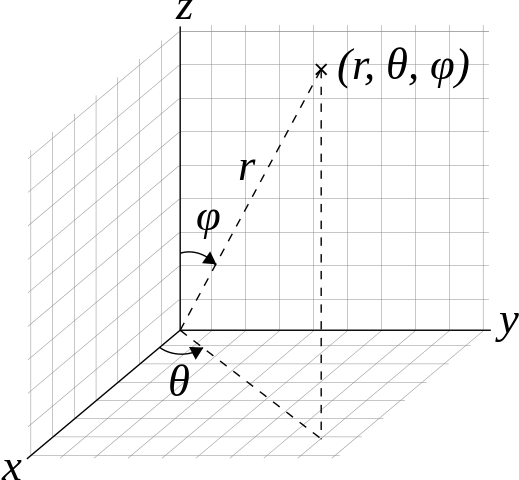
\includegraphics[scale=.2]{spherical.png}
% \end{center}
\begin{equation*}
	\vec{g} :
	\begin{bmatrix}
		x \\
		y \\
		z \\
	\end{bmatrix} =
	\begin{bmatrix}
		\rho \sin \phi \cos \theta \\
		\rho \sin \phi \sin \theta \\
		\rho \cos \phi             \\
	\end{bmatrix}
\end{equation*}
\begin{equation*}
	\rho = \sqrt{x^2 + y^2 + z^2}
\end{equation*}
\begin{equation*}
	\abs{detJ_{\vec{g}}(\vec{u})} = \rho^2 \sin(\phi)
\end{equation*}
\subsection{Coordinate cilindriche}
\begin{equation*}
	\vec{g} :
	\begin{bmatrix}
		x \\
		y \\
		z \\
	\end{bmatrix} =
	\begin{bmatrix}
		r \cos \theta \\
		r \sin \theta \\
		z             \\
	\end{bmatrix}
\end{equation*}
\begin{equation*}
	r = \sqrt{x^2 + y^2}
\end{equation*}
\begin{equation*}
	\abs{detJ_{\vec{g}}(\vec{u})} = r
\end{equation*}
\section{Curve e superfici}
Curva $\gamma:[a,b]\rightarrow\mathbb{R}^n$,\\ $f:A\subset{\mathbb{R}^n}\rightarrow\mathbb{R}$, \\
$F:B\subset\mathbb{R}^n\rightarrow\mathbb{R}^n$
$$ L(\gamma) = \int_{a}^{b} \norm{\gamma'(t)} \dif t$$
$$ \int_{\gamma} f\dif s = \int_a^b f(\gamma(t)) \norm{\gamma'(t)} \dif t$$
$$ \int_\gamma \omega_{F} = \int_\gamma \langle F(\gamma(t)), \gamma'(t)\rangle \dif s = $$\\
$$ = \int_a^b \sum_{i=1}^n\left[F_i(\gamma(t))~\gamma_i'(t)\right] \dif t$$

Superficie S con par. $\phi:D\subset\mathbb{R}^2\rightarrow\mathbb{R}^n$, $\phi(u, v) = (\phi_1, \dots, \phi_n)$\\
$$ Area(S) = \iint_D \norm{\phi_u \wedge \phi_v} \dif u \dif v$$

\section{Teoremi principali}
\begin{itemize}
	\item $f$ differenziabile in $x_0~ \Rightarrow~f$ continua in $x_0 $
	\item \textbf{Teorema del differenziale totale} \\ Derivate parziali di $f$ esistono in un intorno di $x_0$ e sono continue in $x_0~\Rightarrow ~ f$ differenziabile in $x_0$ 
	\item \textbf{Schwarz con due alternative} \\ 1) Derivate seconde miste $f_{xy}$ e $f_{yx}$ di $f$ esistono in un intorno di $x_0$ e sono continue in $x_0~\Rightarrow~f_{xy} = f_{yx}$ in $x_0$
			\\ 2) $f_{xy}$ e $f_{yx}$ esitono nell'intorno e sono differenziabili nel punto $\Rightarrow~_{xy} = f_{yx}$ in $x_0$
	\item \textbf{Lagrange direzionale a valori scalari} 
	\item \textbf{Lagrange direzionale a valori vettori}
	\item $f : A \rightarrow \mathbb{R^m}$ continua, $A$ connesso $\Rightarrow~f(A)$ è connesso
	\item \textbf{Fermat}
	\item \textbf{Teorema sui punti estremali}


\end{itemize}

\end{document}
